\begin{figure}[h!]
    \centering
    \makebox[\textwidth][c]{
    
        \begin{minipage}{0.5\linewidth}
            \centering
            \begin{algorithm}[H]
            \caption{}
            \begin{algorithmic}[1]
            \Require Integer $A$, $B$, Scratchpad memory $S$
            \Ensure Modified scratchpad memory $S$
            \For{$i \leftarrow 1$ to $524288$}
                \State $C \leftarrow \text{AES}(S[A], A)$
                \State $S[A] \leftarrow \text{XOR}(B, C)$
                \State $D \leftarrow S[C]$
                \State $A \leftarrow \text{ADD}(A, \text{MUL}(C, D))$
                \State $S[C] \leftarrow A$
                \State $A \leftarrow \text{XOR}(A, D)$
                \State $B \leftarrow C$
            \EndFor
            \end{algorithmic}
            \end{algorithm}
        \end{minipage}
        
        \hspace{0.05\linewidth}
        
        \begin{minipage}{0.45\linewidth}
            \centering
            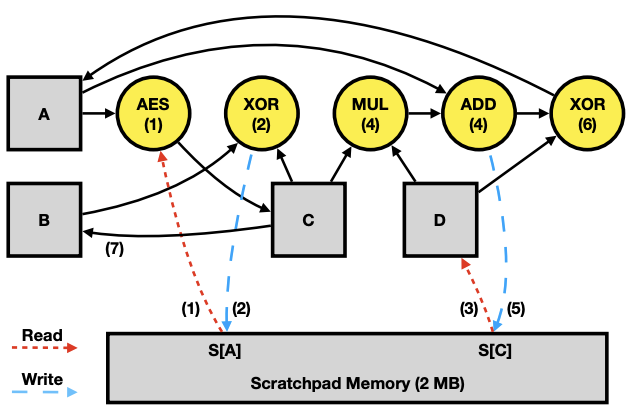
\includegraphics[width=\linewidth]{images/cryptonight.png}
        \end{minipage}
    }
    \caption{Memory-Hard loop dell'algoritmo CryptoNight. \cite{asic_memory_hard}}
    \label{fig:cryptonight-loop}
\end{figure}